%%%%%%%%%%%%%%%%%%%%%%%%%%%%%%%%%%%%%%%%%%%%%%%%%%%%%%%%%%%%%
%% Aufgabe 3; Statische/Dynamische Semantik
%%%%%%%%%%%%%%%%%%%%%%%%%%%%%%%%%%%%%%%%%%%%%%%%%%%%%%%%%%%%%
\chapter{Aufgabe 3}
\label{sec:aufgabe3}

\subsection*{a)}
Sie haben in Aufgabe 2 eine kleine Sprache mit konkreter und abstrakter Syntax definiert.
Lässt sich eine statische Semantik für Ihre abstrakte Syntax angeben?
Erlaubt Ihre konkrete Syntax Formulierungen, die die statische Semantik verletzen?
Ergänzen Sie gegebenenfalls eine statische Semantikprüfung für Ihre Sprache.

Falls Ihre eigene Sprache hinsichtlich statischer Sematik nichts hergibt,
laden Sie die ANTLR4 Java Grammatik herunter und schreiben Sie mit Hilfe der generierten Listener-Klasse eine statische Semantikprüfung,
die sicherstellt, dass ganzzahlige Literale ohne L im Zahlbereich von int und mit L im Zahlbereich von long liegen.

\subsection*{a - Lösung}
\newline
\begin{code}[language=java, caption={ParserListener für statische Syntax}, label={lst:Aufgabe3a}]
public class CreationStatic extends CreationParserBaseListener {

    public static void main(String[] args) throws IOException {
        CreationLexer lexer = new CreationLexer(args.length >= 1 ?
        CharStreams.fromString(args[0]) : CharStreams.fromStream(System.in));
        CreationParser parser = new CreationParser(new CommonTokenStream(lexer));
        ParseTree tree = parser.param();

        if (parser.getNumberOfSyntaxErrors() > 0) {
            System.err.printf("%d error(s) detected%n", parser.getNumberOfSyntaxErrors());
            System.exit(1);
        }

        new ParseTreeWalker().walk(new CreationStatic(), tree);
    }

    @Override
    public void enterParam(CreationParser.ParamContext ctx) {

        if (ctx.start.getType() == CreationParser.NUM) {
            System.out.println("Found a Number: " + ctx.getText());

            var literal = ctx.NUM().getText();

            if (literal.endsWith("L") || literal.endsWith("l")) {
                System.out.print("Expected Long: ");
                long value;
                try {
                    value = Long.parseLong(literal.substring(0, literal.length() - 1));
                } catch (NumberFormatException e) {
                    System.out.println("Bigger than Long!");
                    throw new RuntimeException(e);
                }
                if (value > Integer.MAX_VALUE) {
                    System.out.println("Found Long!");
                } else {
                    System.out.println("Wrong range!");
                }

            } else {
                System.out.print("Expected Integer: ");

                try {
                    Integer.parseInt(literal);
                    System.out.println("Found Integer!");
                } catch (NumberFormatException e) {
                    System.out.println("Wrong range!");
                }
            }
            System.out.println();
        }
    }
}
\end{code}
\newline

Umsetzung der statischen Semantikprüfung mit der ANTLR4 Java Grammatik.
\newline
Beim Parsen wird jeder Paramter mit der \textit{enterParam} Methode des Listeners überprüft, ob dieser ein im Falle einer Zahl, ein Integer oder Long ist.
Dies geschiet indem aus dem Kontext der Regeltyp hergeleitet wird.
Sollte der Typ \textit{NUM} sein, wird überprüft ob der Literalwert mit einem \textit{L} oder \textit{l} für \textit{Long} endet.
Falls dies der Fall ist, wird der Wert in einen Long geparst und überprüft ob dieser größer als der Maximalwert von Integer ist.
Somit ist sichergestellt, dass der Wert im Bereich von Long liegt.
Falls dies nicht der Fall ist, wird der Wert in einen Integer geparst und somit indirekt überprüft ob dieser im Bereich von Integer liegt.
Das Parsen ist jeweils in einem Try-Catch Block, da bei einem zu großen Wert eine \textit{NumberFormatException} geworfen wird.
Dadurch ist gegeben, dass die Wertebereiche stimmen.
\newline
\newline
\newline
\newline
\begin{figure}[h]
	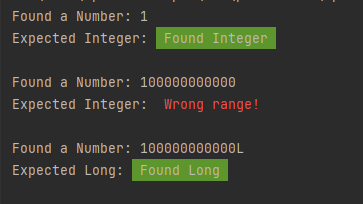
\includegraphics[width=\textwidth]{media/Aufgabe3a_static_output}
	\caption{Ausgabe für: "new Class(1, 100000000000, 100000000000L)"}
	\label{img:Aufgabe3a_output}
\end{figure}
\newline

\subsection*{b)}
Programmieren Sie für Ihre eigene Sprache aus Aufgabe 2 mindestens eine dynamische Semantik.

\subsection*{b - Lösung}
\newline
\begin{code}[language=java, caption={\textit{SillyClass} als Vorgabe für dynamische Semantikprüfung}, label={lst:Aufgabe3b}]
public class SillyClass {
    int x = 0;

    public SillyClass(int x) {
        this.x = x;
    }
}
\end{code}
\newline
In der Aufgabe wird für die vorgegebene \textit{SillyClass} eine dynamische Semantikprüfung implementiert.
\newline
\newline
\textbf{Code}
\begin{code}[language=java, caption={ParserListener für dynamische Semantik}, label={lst:Aufgabe3b}]
public class CreationDynamicAnalyzer extends CreationParserBaseListener {

    static String pre = """
            package u3;

            public class CreationDynamic {
                public static void main(String[] args) {
                    System.out.println(
                    """;
    static String post = """

                    );
                }
            }""";

    StringBuilder sb = new StringBuilder(pre).append("\t\t\t");

    public static void main(String[] args) throws IOException {
        CreationLexer lexer = new CreationLexer(args.length >= 1 ?
                CharStreams.fromString(args[0]) : CharStreams.fromStream(System.in));
        CreationParser parser = new CreationParser(new CommonTokenStream(lexer));
        ParseTree tree = parser.start();

        if (parser.getNumberOfSyntaxErrors() > 0) {
            System.err.printf("%d error(s) detected%n", parser.getNumberOfSyntaxErrors());
            System.exit(1);
        }

        new ParseTreeWalker().walk(new CreationDynamicAnalyzer(), tree);

    }

    @Override
    public void enterExpr(CreationParser.ExprContext ctx) {
        if (ctx.getChildCount() == 6) {

            if (!ctx.getChild(2).getText().equals(SillyClass.class.getSimpleName())) {

                System.out.println(ctx.getChild(2).getText() + " == " + SillyClass.class.getSimpleName());
                throw new RuntimeException("Wrong class name!");
            }
            for (int i = 0; i < ctx.getChildCount(); i++) {
                sb.append(ctx.getChild(i).getText());
            }
            sb.append(post);

            if (ctx.params().param().size() != 1) {
                throw new RuntimeException("Wrong number of parameters!");
            }

            try {
                FileWriter myWriter = new FileWriter("./src/u3/CreationDynamic.java");
                myWriter.write(sb.toString());
                myWriter.close();
                System.out.println("Successfully wrote to the file.");
            } catch (IOException e) {
                System.out.println("An error occurred.");
                e.printStackTrace();
            }
        }
    }
}
\end{code}

In der \textit{enterExpr} Methode wird dynamisch überprüft ob die Klasse, die erstellt werden soll, die richtige ist.
Dabei stellen wir zuerst sicher, dass die Anzahl der Parameter stimmt, welche bei der Klasse \textit{SillyClass} nur ein Parameter ist
und somit die Anzahl an Kindern des Kontextes 6 ist.
\newline
\textit{Siehe Parser: expr : KEYWORD WS NAME PAR\_OPEN params PAR\_CLOSE ;}
\newline
Danach wird abgefangen, wenn der Klassenname nicht der Klasse \textit{SillyClass} entspricht.
Im selben Stil wird abgefragt ob die Anzahl der Parameter stimmt.
Erst wenn diese Bedingungen erfüllt sind, wird der Code in eine Datei geschrieben.
Dabei sind \textit{pre} und \textit{post} Strings, welche den Code vor und nach dem erstellen eines \textit{SillyClass} Objektes enthalten.
\newline
\newline
\textbf{Entstandener Code}
\begin{code}[language=java, caption={Erstellt für Input: \textit{new SillyClass(22)}}, label={lst:Aufgabe3b}]
public class CreationDynamic {
    public static void main(String[] args) {
        System.out.println(
			new SillyClass(22)
        );
    }
}
\end{code}
\newline
\textbf{Ausgabe bei falscher Klasse}
\begin{figure}[h]
    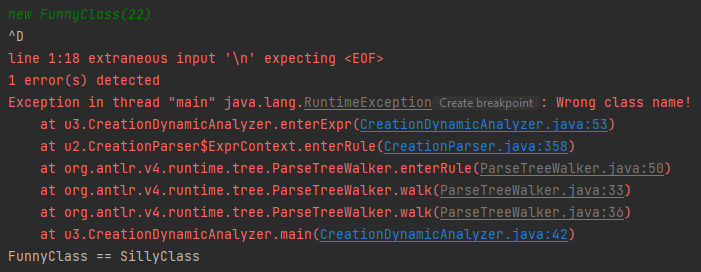
\includegraphics[width=\textwidth]{media/Aufgabe3b_wrong_output}
    \caption{Ausgabe für: \textit{new FunnyClass(22)}}
    \label{img:Aufgabe3b_output}
\end{figure}
